\section{Simulation}
\label{sec:simulation}
After understanding how the filter worked in theory, its properties and after getting an overview of how it was being implemented and which considerations were being made, we implemented a virtual prototype MATLAB to quickly explore the design space. We used this prototype to refine our understanding of the algorithm and to make decisions in view of the future vhdl implementation. Furthermore, we were able to use this virtual prototype to create input stimuli and the expected responses, i.e. a test bench, which will be fed to the VHDL implementation for verification.
%We have used simulation tools, including MATLAB and VHDL testbench, to validate our Goertzel Filter design. To guarantee proper functionality, the MATLAB simulation produce stimulus data and expected outputs, while the VHDL testbench compares the filter's output with anticipated outcomes.
We created a total of 57 input signals, whose length is equal to $N = 100$. The signals have the following characteristics.
\begin{itemize}
    \item Sine Waves in 5, 49, 50, 51 and 200 kHz, with phase angles in 0°, 30°, 45°, 90°, 120° respectively
    \item Rectangular Waves in 10, 16, 50 and 200 kHz, with phase angles in 0°, 30°, 45°, 90°, 120° respectively
    \item Triangle Waves in 50 kHz, with phase angles in 0° and 90° respectively
    \item Sine Waves in 5, 49, 50, 51 and 200 kHz combined, with phase angles in 0°, 30°, 45°, 90°, 120° respectively
    \item Rectangular Waves in 10, 16, 50 and 200 kHz combined, with phase angles in 0°, 30°, 45°, 90°, 120° respectively
\end{itemize}

\subsection{MATLAB Simulation with floating-point numbers}  \label{sec:matlab-float}

Following the specifications, we scaled and applied an offset to the input signals, such that they are expressed in terms of offset binary numbers ranging from $0$ to $2^{14} - 1$. The conversion from the original signals (that range from $-1$ to $1$) to offset binary numbers has been achieved with following process:

\lstset{language=Matlab}
\begin{figure}[H] \begin{lstlisting}
function output = scaleToInt(input, bit_len, input_swing)
    % Scale the waveforms to the range of 2^(bit_len - 1) +/- 2^input_swing
    scaled = (2 ^ bit_len - 1) / 2 + input * (2 ^ input_swing - 1) / 2;
    % Convert the scaled waveforms to (bit_len)-bit unsigned integers
    output = int32(round(scaled));
end
\end{lstlisting}
\caption{Code snippet for offset binary conversion}
\end{figure}

The signals are written into files and to be read by the VHDL testbench, which will be introduced in Section n. \ref{sec:testbench}.
We developed our implemention of the Goertzel Filter according to Equations n. \ref{eq:UPDATE} and n. \ref{eq:yn2}, which we used to derive the results of different input signals, depicted in in Fig. n. \ref{fig:gf_sim}.

\begin{figure}[H]
    \centering
    \begin{subfigure}[b]{\textwidth}
        \centering
        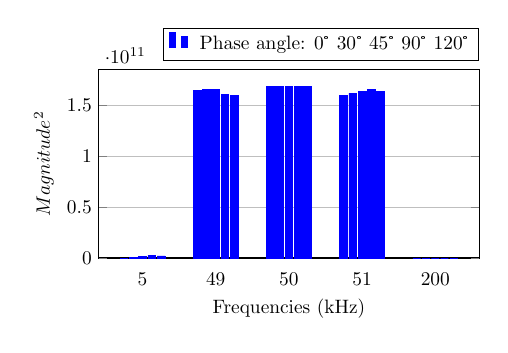
\begin{tikzpicture}[scale = 0.7]
          \begin{axis}[
              width  = 0.7*\textwidth,
              height = 5cm,
              major x tick style = transparent,
              ybar=2*\pgflinewidth,
              bar width=4pt,
              ymajorgrids = true,
              xlabel = {Frequencies (kHz)},
              ylabel = {$Magnitude^2$},
              symbolic x coords={5, 49, 50, 51, 200},%, combined},
              xtick = data,
              scaled x ticks = true,
              scaled y ticks = true,
              enlarge x limits=0.15,
              ymin=0,
              legend cell align=left,
              legend style={
                  at={(1,1.05)},
                  anchor=south east,
                  column sep=1ex
                },
              extra y ticks = 0.4,
              extra y tick labels={},
              extra y tick style={grid=major,major grid style={thick,draw=black}}
            ]
            \addplot[style={blue,fill=blue,mark=none}]
            coordinates {(5, 28165288) (49, 164300582087) (50, 167754581071) (51, 159204915664) (200, 19) %(combined, 55316152356)
            };
        
             %\addplot[style={black,fill=red,mark=none}]
             %coordinates {(5, 27262976) (49, 164186030080) (50, 167786840064) (51, 159184322560) (200, 0)};
        
            \addplot[style={blue,fill=blue,mark=none}]
            coordinates {(5, 682813699) (49, 165638701140) (50, 167757951221) (51, 161622013902) (200, 6) %(combined, 57679231120)
            };
        
            \addplot[style={blue,fill=blue,mark=none}]
            coordinates {(5, 1368984191) (49, 165006710536) (50, 167745947887) (51, 163313161637) (200, 14) %(combined, 58261386167)
            };
        
            \addplot[style={blue,fill=blue,mark=none}]
            coordinates {(5, 2796749553) (49, 160349176237) (50, 167748444133) (51, 165437419087) (200, 19) %(combined, 56341860579)
            };
        
            \addplot[style={blue,fill=blue,mark=none}]
            coordinates {(5, 2142148654) (49, 159011970308) (50, 167756010813) (51, 163022198679) (200, 29) %(combined, 53976111895)
            };
        
            \legend{Phase angle: 0° 30° 45° 90° 120°}
            \addlegendimage{my legend}
          \end{axis}
        \end{tikzpicture}
        \caption{Sine waves}
        \label{fig:gf_sim_sine}
    \end{subfigure}

    %\vspace{0.5cm}
    
    \begin{subfigure}[b]{0.6\textwidth}
        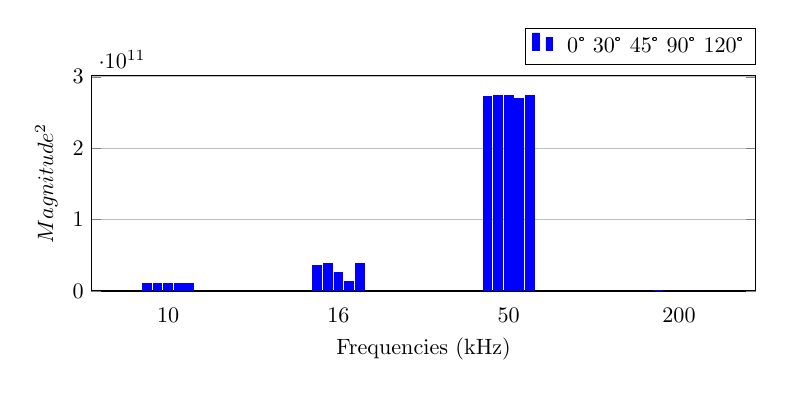
\begin{tikzpicture}[scale = 0.8]
          \begin{axis}[
              width  = \textwidth,
              height = 5cm,
              major x tick style = transparent,
              ybar=2*\pgflinewidth,
              bar width=4pt,
              ymajorgrids = true,
              xlabel = {Frequencies (kHz)},
              ylabel = {$Magnitude^2$},
              symbolic x coords={10, 16, 50, 200},%, combined},
              xtick = data,
              scaled x ticks = true,
              scaled y ticks = true,
              enlarge x limits=0.15,
              ymin=0,
              legend cell align=left,
              legend style={
                  at={(1,1.05)},
                  anchor=south east,
                  column sep=1ex
                },
              extra y ticks = 0.4,
              extra y tick labels={},
              extra y tick style={grid=major,major grid style={thick,draw=black}}
            ]
            \addplot[style={blue,fill=blue,mark=none}]
            coordinates {(10, 10967862060) (16, 35190107208) (50, 271780927294) (200, 268402689) %(combined, 39636235246)
            };
        
            \addplot[style={blue,fill=blue,mark=none}]
            coordinates {(10, 10967862060) (16, 38711007665) (50, 274196551495) (200, 0) %(combined, 27759917661)
            };
        
            \addplot[style={blue,fill=blue,mark=none}]
            coordinates {(10, 10967862060) (16, 25835512141) (50, 274196551495) (200, 0) 
            %(combined, 19477158285)
            };
        
            \addplot[style={blue,fill=blue,mark=none}]
            coordinates {(10, 10967862060) (16, 13709827575) (50, 269902108471) (200, 0) 
            %(combined, 16577256943)
            };
        
            
            \addplot[style={blue,fill=blue,mark=none}]
            coordinates {(10, 10967862060) (16, 38711007665) (50, 274196551495) (200, 0) 
            %(combined, 6703613435)
            };
        
            \legend{0° 30° 45° 90° 120°}
            \addlegendimage{my legend}
          \end{axis}
        \end{tikzpicture}
        \caption{Rectangular waves}
    \end{subfigure}
    \hfill
    \begin{subfigure}[b]{0.35\textwidth}
        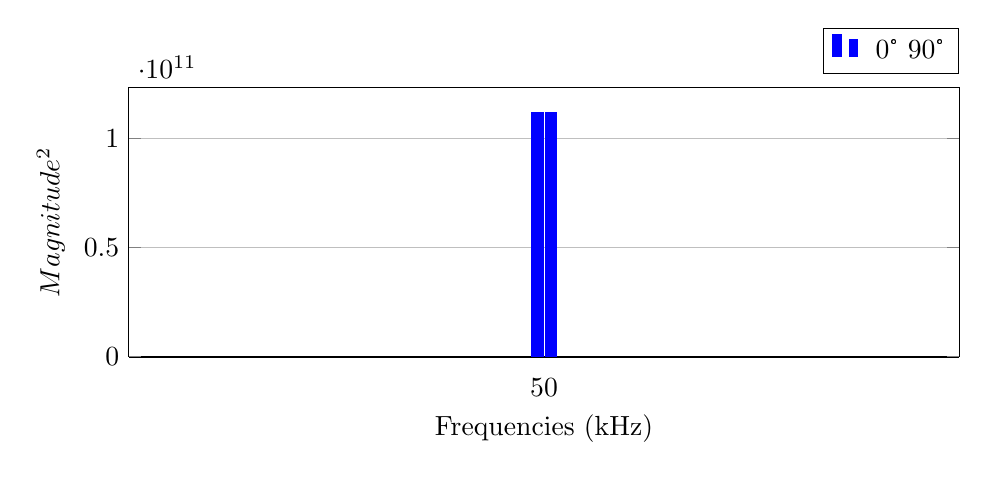
\begin{tikzpicture}
          \begin{axis}[
              width  = \textwidth,
              height = 5cm,
              major x tick style = transparent,
              ybar=2*\pgflinewidth,
              bar width=4pt,
              ymajorgrids = true,
              xlabel = {Frequencies (kHz)},
              ylabel = {$Magnitude^2$},
              symbolic x coords={50},
              xtick = data,
              scaled x ticks = true,
              scaled y ticks = true,
              enlarge x limits=0.15,
              ymin=0,
              legend cell align=left,
              legend style={
                  at={(1,1.05)},
                  anchor=south east,
                  column sep=1ex
                },
              extra y ticks = 0.4,
              extra y tick labels={},
              extra y tick style={grid=major,major grid style={thick,draw=black}}
            ]
            \addplot[style={blue,fill=blue,mark=none}]
            coordinates {(50, 112045721003)};
        
            \addplot[style={blue,fill=blue,mark=none}]
            coordinates {(50, 112045721002)};
        
            \legend{0° 90°}
            \addlegendimage{my legend}
          \end{axis}
        \end{tikzpicture}
        \caption{Triangle waves}
    \end{subfigure}
    
    \caption{Results of MATLAB simulation with floating-point numbers}
    \label{fig:gf_sim}
\end{figure}

The obtained result aligns with expectations, as the Goertzel filter exhibits a high magnitude response only for waves containing a component around 50 kHz, which corresponds to the signal frequency to detect ($F_k$).
As shown in Fig. n. \ref{fig:gf_sim_sine}, the filter in this design can barely differentiate between 49, 50 and 51 kHz signals. By changing the number of samples, we concluded that the frequency resolution is depending on the number of samples ($N$), as demonstrated that by the fact that, for example, when $N = 500$, the magnitudes for 50 kHz signals are much different from those for 49 and 51 kHz (Fig. n. \ref{fig:gf_sim_N500}), and the difference between those is much more recognizable.

\begin{figure}[H]
  \centering
  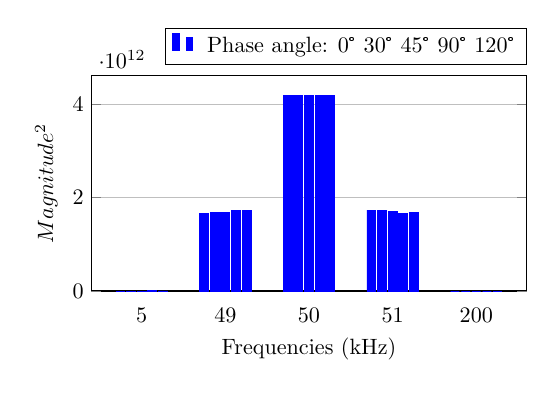
\begin{tikzpicture}[scale = 0.8]
    \begin{axis}[
        width  = 0.7*\textwidth,
        height = 5cm,
        major x tick style = transparent,
        ybar=2*\pgflinewidth,
        bar width=4pt,
        ymajorgrids = true,
        xlabel = {Frequencies (kHz)},
        ylabel = {$Magnitude^2$},
        symbolic x coords={5, 49, 50, 51, 200},%, combined},
        xtick = data,
        scaled x ticks = true,
        scaled y ticks = true,
        enlarge x limits=0.15,
        ymin=0,
        legend cell align=left,
        legend style={
            at={(1,1.05)},
            anchor=south east,
            column sep=1ex
          },
        extra y ticks = 0.4,
        extra y tick labels={},
        extra y tick style={grid=major,major grid style={thick,draw=black}}
      ]
      \addplot[style={blue,fill=blue,mark=none}]
      coordinates {(5, 28136055) (49, 1666618598937) (50, 4193875917772) (51, 1732388606682) (200, 205) 
      %(combined, 167767402016)
      };

      \addplot[style={blue,fill=blue,mark=none}]
      coordinates {(5, 683029058) (49, 1674052576567) (50, 4193942960824) (51, 1725444346577) (200, 41) 
      %(combined, 175769719174)
      };
  
      \addplot[style={blue,fill=blue,mark=none}]
      coordinates {(5, 1369507272) (49, 1689292248901) (50, 4193627387892) (51, 1710630899751) (200, 59) 
      %(combined, 177898066729)
      };

      \addplot[style={blue,fill=blue,mark=none}]
      coordinates {(5, 2796634597) (49, 1733120151328) (50, 4193826613449) (51, 1667358625940) (200, 61) 
      %(combined, 172045669337)
      };
  
      \addplot[style={blue,fill=blue,mark=none}]
      coordinates {(5, 2141985241) (49, 1725657357466) (50, 4193909153782) (51, 1674273740527) (200, 124) 
      %(combined, 164047439042)
      };
  
      \legend{Phase angle: 0° 30° 45° 90° 120°}
      \addlegendimage{my legend}
    \end{axis}
  \end{tikzpicture}
    
  \caption{Results of MATLAB simulation of sine waves, N = 500}
  \label{fig:gf_sim_N500}
\end{figure}

The magnitudes of multi-tone waves with all the frequencies combined are lower than those of single-tone waves in 50 kHz. This is because the multi-tone waves are normalized to $0$ to $2^{14} - 1$, hence their components corresponding to 50 kHz is smaller than those single-tone waves.

\subsection{MATLAB Simulation with integers and LSB truncation}  \label{sec:matlab-int}

Since we aim to synthetize our VHDL implementation in real hardware and we aim to develop it in a way that is efficient in both performance and resources used, we analysed the difference between representing numbers as integers and as floating points.
To do so, we created another version of the Goertzel filter that used integers instead of floating-point numbers, with least significant bits (LSB) truncated to mimic what we would need to do in the VHDL implementation. The purpose of this version is to verify that any deviation between the MATLAB and VHDL results is attributed to the expected truncation error resulting from the filter design, rather than errors arising from mistakes in the VHDL implementation.
LSB are truncated as demonstrated in Fig. n. \ref{code:lsb_trunc}, where the value of $s(n)$ first divided by $2^{LSB\_TRUNC}$, next is passed to the \texttt{floor()} function, which converts the result of the expression inside to the nearest lower integer. The result is then multiplied by $2^{LSB\_TRUNC}$, effectively quantizing the result to 18 bits, as required by the specifications in Table n. \ref{tab:specifications}.

\lstset{language=Matlab}
\begin{figure}[H] \begin{lstlisting}
LSB_TRUNC = 5; % internal data's LSB truncated
...
s(n) = floor(double(signal(n) + multi_prod - sprev2) / 2 ^ LSB_TRUNC) * (2 ^ LSB_TRUNC);
\end{lstlisting}
\caption{Code snippet for LSB truncation}
\label{code:lsb_trunc}
\end{figure}

We compared the results of the two functions, as shown in Fig. n. \ref{fig:gf_sim_int} and Table \ref{tab:result}. The differences between the 2 versions is at most $1.2 \times 10^8$, and considering that the output is in the magnitude of $10^{11}$, the error is less than $0.1\%$, which can be considered acceptable in view of the reduced complexity given by avoiding floating numbers.
The outputs are again written into files and to be read by the VHDL testbench, which will be further discussed in Section n. \ref{sec:testbench}.

\begin{figure}[H]
  \centering
  \begin{subfigure}[b]{\textwidth}
    \centering
    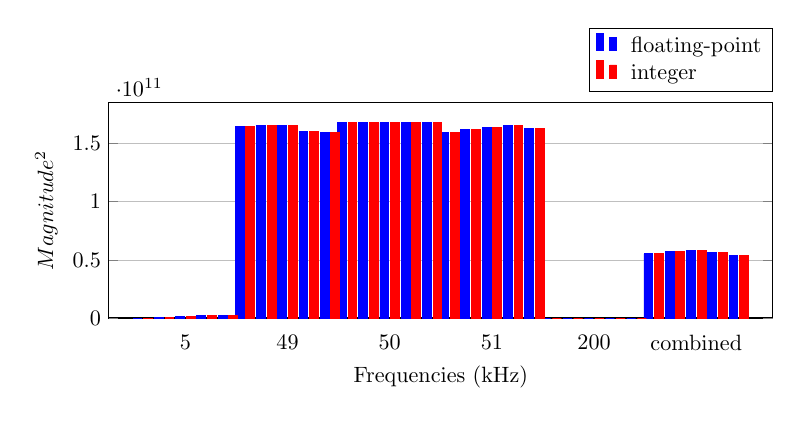
\begin{tikzpicture}[scale = 0.8]
      \begin{axis}[
          width  = \textwidth,
          height = 5cm,
          major x tick style = transparent,
          ybar=2*\pgflinewidth,
          bar width=4pt,
          ymajorgrids = true,
          xlabel = {Frequencies (kHz)},
          ylabel = {$Magnitude^2$},
          symbolic x coords={5, 49, 50, 51, 200, combined},
          xtick = data,
          scaled x ticks = true,
          scaled y ticks = true,
          enlarge x limits=0.15,
          ymin=0,
          legend cell align=left,
          legend style={
              at={(1,1.05)},
              anchor=south east,
              column sep=1ex
            },
          extra y ticks = 0.4,
          extra y tick labels={},
          extra y tick style={grid=major,major grid style={thick,draw=black}}
        ]
        \addplot[style={blue,fill=blue,mark=none}]
        coordinates {(5, 28165288) (49, 164300582087) (50, 167754581071) (51, 159204915664) (200, 19) (combined, 55316152356)};
        \addplot[style={red,fill=red,mark=none}]
        coordinates {(5, 27262976) (49, 164186030080) (50, 167786840064) (51, 159184322560) (200, 0) (combined, 55293509632)};
        \addplot[style={blue,fill=blue,mark=none}]
        coordinates {(5, 682813699) (49, 165638701140) (50, 167757951221) (51, 161622013902) (200, 6) (combined, 57679231120)};
        \addplot[style={red,fill=red,mark=none}]
        coordinates {(5, 679477248) (49, 165589024768) (50, 167845560320) (51, 161633796096) (200, 0) (combined, 57680068608)};
        \addplot[style={blue,fill=blue,mark=none}]
        coordinates {(5, 1368984191) (49, 165006710536) (50, 167745947887) (51, 163313161637) (200, 14) (combined, 58261386167)};
        \addplot[style={red,fill=red,mark=none}]
        coordinates {(5, 1365245952) (49, 165033279488) (50, 167784742912) (51, 163238117376) (200, 0) (combined, 58294534144)};
        \addplot[style={blue,fill=blue,mark=none}]
        coordinates {(5, 2796749553) (49, 160349176237) (50, 167748444133) (51, 165437419087) (200, 19) (combined, 56341860579)};
        \addplot[style={red,fill=red,mark=none}]
        coordinates {(5, 2791309312) (49, 160327270400) (50, 167723925504) (51, 165435932672) (200, 0) (combined, 56329502720)};
        \addplot[style={blue,fill=blue,mark=none}]
        coordinates {(5, 2142148654) (49, 159011970308) (50, 167756010813) (51, 163022198679) (200, 29) (combined, 53976111895)};
        \addplot[style={red,fill=red,mark=none}]
        coordinates {(5, 2139095040) (49, 159020744704) (50, 167832977408) (51, 163108093952) (200, 0) (combined, 53953429504)};
        \legend{floating-point, integer}
        \addlegendimage{my legend}
      \end{axis}
    \end{tikzpicture}
    \caption{Sine waves}
  \end{subfigure}


  \begin{subfigure}[b]{\textwidth}
  \centering
    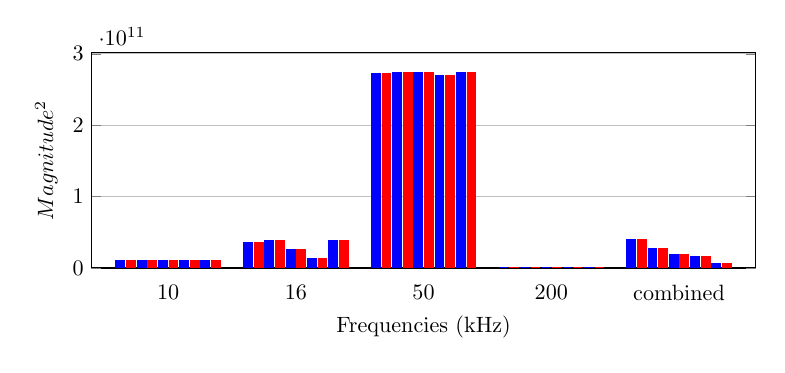
\begin{tikzpicture}[scale = 0.8]
      \begin{axis}[
          width  = \textwidth,
          height = 5cm,
          major x tick style = transparent,
          ybar=2*\pgflinewidth,
          bar width=4pt,
          ymajorgrids = true,
          xlabel = {Frequencies (kHz)},
          ylabel = {$Magnitude^2$},
          symbolic x coords={10, 16, 50, 200, combined},
          xtick = data,
          scaled x ticks = true,
          scaled y ticks = true,
          enlarge x limits=0.15,
          ymin=0,
          legend cell align=left,
          legend style={
              at={(1,1.05)},
              anchor=south east,
              column sep=1ex
            },
          extra y ticks = 0.4,
          extra y tick labels={},
          extra y tick style={grid=major,major grid style={thick,draw=black}}
        ]
        \addplot[style={blue,fill=blue,mark=none}]
        coordinates {(10, 10967862060) (16, 35190107208) (50, 271780927294) (200, 268402689) (combined, 39636235246)};
        \addplot[style={red,fill=red,mark=none}]
        coordinates {(10, 10951327744) (16, 35108421632) (50, 271730081792) (200, 266338304) (combined, 39696990208)};
        \addplot[style={blue,fill=blue,mark=none}]
        coordinates {(10, 10967862060) (16, 38711007665) (50, 274196551495) (200, 0) (combined, 27759917661)};
        \addplot[style={red,fill=red,mark=none}]
        coordinates {(10, 10984882176) (16, 38669385728) (50, 274141806592) (200, 0) (combined, 27736932352)};
        \addplot[style={blue,fill=blue,mark=none}]
        coordinates {(10, 10967862060) (16, 25835512141) (50, 274196551495) (200, 0) (combined, 19477158285)};
        \addplot[style={red,fill=red,mark=none}]
        coordinates {(10, 10974396416) (16, 25813843968) (50, 274080989184) (200, 0) (combined, 19480444928)};
        \addplot[style={blue,fill=blue,mark=none}]
        coordinates {(10, 10967862060) (16, 13709827575) (50, 269902108471) (200, 0) (combined, 16577256943)};
        \addplot[style={red,fill=red,mark=none}]
        coordinates {(10, 10982785024) (16, 13719568384) (50, 269859422208) (200, 0) (combined, 16571695104)};
        \addplot[style={blue,fill=blue,mark=none}]
        coordinates {(10, 10967862060) (16, 38711007665) (50, 274196551495) (200, 0) (combined, 6703613435)};
        \addplot[style={red,fill=red,mark=none}]
        coordinates {(10, 10970202112) (16, 38646317056) (50, 274141806592) (200, 0) (combined, 6696206336)};
      \end{axis}
    \end{tikzpicture}
    \caption{Rectangular waves}
  \end{subfigure}

  \vspace{0.5cm}

  \begin{subfigure}[b]{0.5\textwidth}
    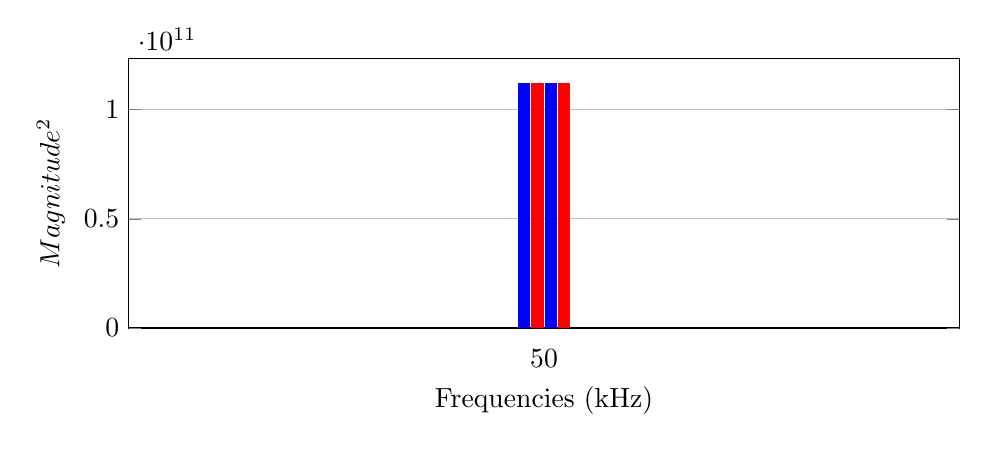
\begin{tikzpicture}
      \begin{axis}[
          width  = \textwidth,
          height = 5cm,
          major x tick style = transparent,
          ybar=2*\pgflinewidth,
          bar width=4pt,
          ymajorgrids = true,
          xlabel = {Frequencies (kHz)},
          ylabel = {$Magnitude^2$},
          symbolic x coords={50},
          xtick = data,
          scaled x ticks = true,
          scaled y ticks = true,
          enlarge x limits=0.15,
          ymin=0,
          legend cell align=left,
          legend style={
              at={(1,1.05)},
              anchor=south east,
              column sep=1ex
            },
          extra y ticks = 0.4,
          extra y tick labels={},
          extra y tick style={grid=major,major grid style={thick,draw=black}}
        ]
        \addplot[style={blue,fill=blue,mark=none}]
        coordinates {(50, 112045721003)};
        \addplot[style={red,fill=red,mark=none}]
        coordinates {(50, 112042442752)};
        \addplot[style={blue,fill=blue,mark=none}]
        coordinates {(50, 112045721002)};
        \addplot[style={red,fill=red,mark=none}]
        coordinates {(50, 112059219968)};
      \end{axis}
    \end{tikzpicture}
    \caption{Triangle waves}
  \end{subfigure}

  \caption{Results of MATLAB simulation with integers and LSB truncation}
  \label{fig:gf_sim_int}
\end{figure}

